\chapter{Аналитический раздел}

\section{Алгоритм шифрования <<DES>>}

\textbf{DES} (Data Encryption Standard) \cite{Enigma} --- это симметричный шифровальный алгоритм, разработанный в 1970-х годах, который использует блочное шифрование с фиксированной длиной блока в 64 бита. Основные шаги и логика работы DES:

1. \textbf{Начальная перестановка} (Initial Permutation):
Исходный текст (64 бита) проходит через начальную перестановку, где биты переставляются в определенном порядке согласно предопределенной таблице перестановок.

2. \textbf{Раунды шифрования} (Rounds):
DES состоит из 16 раундов шифрования, каждый из которых включает несколько шагов:
\begin{itemize}
	\item[---] \textbf{Расширение} (Expansion): 32-битный входной блок расширяется до 48 бит путем перестановки и дублирования некоторых битов.
	\item[---] \textbf{Ключ раунда} (Round Key): к 48-битному расширенному блоку применяется 48-битный ключ раунда, полученный из основного ключа DES.
	\item[---] \textbf{Скремблирование} (Substitution): 48-битный блок проходит через S-блоки (Substitution-boxes), которые заменяют блоки по 6 бит на блоки по 4 бита с использованием заранее определенных таблиц замен.
	\item[---] \textbf{Перестановка} (Permutation):  после замены, полученный блок по 32 бита проходит через таблицу перестановки, которая перемешивает биты в блоке.
	\item[---] \textbf{Обработка ключа} (Key Mixing): к полученному блоку применяется операция XOR с ключом раунда для обеспечения взаимодействия ключа и данных.
\end{itemize}

3. \textbf{Завершающая перестановка} (Final Permutation):
После 16 раундов, 64-битный блок проходит через последнюю перестановку, обратную начальной перестановке, чтобы получить зашифрованный текст.

Основным элементом DES является ключ, который состоит из 56 бит, и который используется для генерации ключей раунда. Ключ разбивается на две половины, и каждая половина сдвигается влево на определенное количество бит в зависимости от номера раунда. Затем, из полученных половинок формируется ключ раунда.

Таким образом, DES использует комбинацию перестановок, замен и операций XOR для шифрования данных. Эти шаги повторяются 16 раз, в каждом раунде используется уникальный ключ. Результат --- зашифрованный блок данных, который без знания правильного ключа практически невозможно расшифровать.

Алгоритм шифрования DES может использоваться в следующих режимах.

\begin{enumerate}
	\item[1.] \textbf{ECB} (Electronic Code Book) --- режим «электронной кодовой книги» (простая замена);
	\item[2.] \textbf{CBC} (Cipher Block Chaining) --- режим сцепления блоков;
	\item[3.] \textbf{CFB} (Cipher Feed Back) --- режим обратной связи по шифротексту;
	\item[4.] \textbf{OFB} (Output Feed Back) --- режим обратной связи по выходу.
\end{enumerate}

\chapter{Конструкторская часть}

\section{Разработка алгоритма}

На рисунке \ref{fig:algo} представлена схема алгоритма шифрования DES.

\begin{figure}[h!]
	\centering
	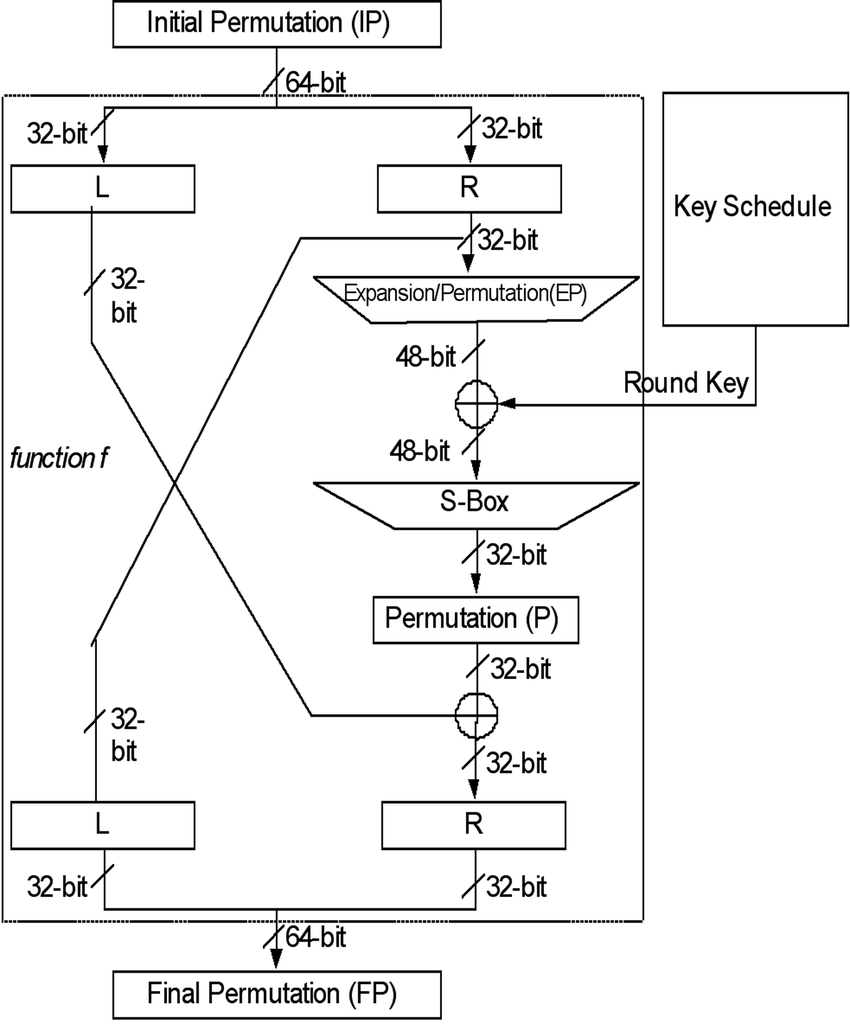
\includegraphics[width=0.85\textwidth]{img/des.png}
	\caption{Схемы алгоритма DES}
	\label{fig:algo}
\end{figure}
\clearpage
